\documentclass[12pt,a4paper]{report}

% Packages
\usepackage{geometry}
\usepackage{fancyhdr}
\usepackage{setspace}
\usepackage{titlesec}
\usepackage{graphicx}
\usepackage{lipsum} 
\usepackage{caption}
\usepackage{listings}
\usepackage{enumitem}
\usepackage{amsmath}
\usepackage{multirow}
\usepackage{pgfplots}
\pgfplotsset{width=10cm,compat=1.17}
\usepackage[hidelinks]{hyperref}
\usepackage[numbers]{natbib}

% Define a new environment for numbered steps
\newenvironment{codedstep}[1][]
  {\begin{enumerate}[label=Step \arabic*:]}
  {\end{enumerate}}


\usepackage{background}
\usepackage{tikz}
\usetikzlibrary{calc}

% Define border style
\newcommand{\PageBorder}{%
    \begin{tikzpicture}[remember picture,overlay]
        \draw[line width=1mm] ($(current page.north west)+(1cm,-1cm)$) rectangle ($(current page.south east)+(-1cm,1cm)$);
    \end{tikzpicture}%
}

% Apply border to all pages
\backgroundsetup{%
    angle=0,
    scale=1,
    color=black,
    opacity=1,
    contents={%
        \PageBorder%
    }
}

% Set page margins
\geometry{top=1in, bottom=1in, left=1in, right=1in}

% Page numbering format
\pagestyle{fancy}
\fancyhf{}
\rfoot{\thepage}
\renewcommand{\headrulewidth}{0pt}

% Chapter and Section formatting
\titleformat{\chapter}[display]
  {\normalfont\fontsize{14}{16}\selectfont\bfseries\centering}{\MakeUppercase{\chaptertitlename}\ \thechapter}{20pt}{\fontsize{14}{16}\selectfont\bfseries}
\titleformat{\section}
  {\normalfont\fontsize{12}{14}\selectfont\bfseries}{\thesection}{1em}{}
\titleformat{\subsection}
  {\normalfont\fontsize{12}{14}\selectfont\bfseries}{\thesubsection}{1em}{}
\titleformat{\subsubsection}
  {\normalfont\fontsize{12}{14}\selectfont\bfseries}{\thesubsubsection}{1em}{}

% Table of Contents formatting
\makeatletter
\renewcommand*\l@chapter[2]{%
  \ifnum \c@tocdepth >\m@ne
    \addpenalty{-\@highpenalty}%
    \vskip 1.0em \@plus\p@
    \setlength\@tempdima{1.5em}%
    \begingroup
      \parindent \z@ \rightskip \@pnumwidth
      \parfillskip -\@pnumwidth
      \leavevmode \bfseries
      \advance\leftskip\@tempdima
      \hskip -\leftskip
      #1\nobreak\hfil \nobreak\hb@xt@\@pnumwidth{\hss #2}\par
      \penalty\@highpenalty
    \endgroup
  \fi}

\renewcommand*\l@section{\@dottedtocline{1}{0em}{2.3em}}
\renewcommand*\l@subsection{\@dottedtocline{2}{2.3em}{3.2em}}
\renewcommand*\l@subsubsection{\@dottedtocline{3}{5.5em}{4.1em}}
\renewcommand*\l@paragraph{\@dottedtocline{4}{8.6em}{5em}}
\renewcommand*\l@subparagraph{\@dottedtocline{5}{12em}{6em}}
\makeatother

% Title Page
\begin{document}
\begin{titlepage}
    \centering
    
    % Title
    {\Huge \bfseries{AI – Algorithms Application on Alibaba Financial Dataset}\par}
    \vspace{1cm}
    {\large A report submitted in partial fulfillment of the requirements for\par}
    {\large\itshape Event 2 of the course of \par}
    \vspace{1cm}
    {\Large\bfseries Artificial Intelligence (20CB630)\par}  % 
    \vspace{1cm}
    {\large by\par}
    \vspace{0.5cm}
    \begin{table}[htbp]
    \centering
    \begin{tabular}{|c|c|}
        \hline
        \textbf{Student Name} & \textbf{USN No} \\
        \hline
        G Rutvik Sharma & 01JST21CB012 \\
        \hline
        Sai Sujith B & 01JST21CB033 \\
        \hline
        Sayed Afnan Khazi & 01JST21CB036 \\
        \hline
        Venkat Bhaskar K & 01JST21CB049 \\
        \hline
    \end{tabular}
\end{table}
\vspace{2cm}

\noindent
\underline{Under the supervision of} \\
\vspace{0.5cm}
Dr. S P Shiva Prakash \\
Professor \& HOD \\
Department of I S \& E \\
JSS S \& T University, Mysuru.

    \vspace{2cm}
    % University Logo
    
\includegraphics[width=0.5\textwidth]{jssstulogo.jpg}\\
    \vspace{1cm}
    % Department and University
    {\Large\bfseries Department of Information Science and Engineering\par}
    {\Large\bfseries JSS Science and Technology University \par}
    {\Large\bfseries 2023-24\par}
\end{titlepage}

% Preliminaries
% Table of Contents 
\tableofcontents

\clearpage

\pagenumbering{arabic} % Start page numbering from arabic numerals
\setcounter{page}{1}

% Abstract
\chapter*{Abstract}
\addcontentsline{toc}{chapter}{Abstract}
\begin{spacing}{1.5}
In today’s dynamic and data-driven business environment, accurately analysing financial data is essential for making informed decisions and maintaining a competitive edge. Machine learning algorithms offer powerful tools for evaluating financial performance, predicting future trends, and uncovering hidden patterns within data. This report focuses on the application of six prominent machine learning algorithms to evaluate financial data and determine their efficacy in performance evaluation - 
\begin{enumerate}
    \item Support Vector Machines (SVM)
    \item K-Nearest Neighbors (KNN)
    \item Decision Trees (DT)
    \item Random Forests (RF)
    \item Artificial Neural Networks (ANN)
    \item Reinforcement Learning (RL)
\end{enumerate}

\end{spacing}
\clearpage


% Main content
\chapter{Introduction}
% Include your Introduction content here.
\begin{spacing}{1.5}
Here, let's discuss each algorithm in detail.
\begin{itemize}
 \item\underline{\textbf{Support Vector Machines (SVM)}} \\
Support Vector Machines (SVM) are supervised learning models used for classification and regression by finding the optimal hyperplane that separates data points of different classes with the maximum margin. SVM is particularly effective in high-dimensional spaces and when the number of dimensions exceeds the number of samples. Implementing SVM involves selecting a suitable kernel (e.g., linear, polynomial, radial basis function), training the model on labelled data, and using the trained model to predict outcomes on new data. The resulting confusion matrix generated by SVM highlights the true positive, true negative, false positive, and false negative predictions, helping evaluate the classifier’s accuracy and other performance metrics.
\\
\item\underline{\textbf{K-Nearest Neighbors (KNN)}} \\
K-Nearest Neighbors (KNN) is an instance-based learning algorithm that classifies data points based on the majority class among the k-nearest neighbours. KNN is non-parametric and lazy, meaning it makes no assumptions about the data distribution and does not perform any generalisation during training. Implementing KNN involves storing all training examples, choosing the number of neighbours (k), calculating the distance between the query instance and all training samples, and predicting the label based on the majority vote of the nearest neighbours. The confusion matrix for KNN provides insights into its classification performance, showing how well the algorithm distinguishes between different classes based on the nearest neighbours.
\\
\item\underline{\textbf{Decision Trees (DT)}} \\
Decision Trees (DT) are non-parametric supervised learning methods used for classification and regression by splitting the data into subsets based on the value of input features, forming a tree-like model of decisions. Implementing DT involves selecting criteria for splitting (e.g., Gini impurity or information gain), growing the tree by recursively splitting nodes, and pruning to avoid overfitting. The confusion matrix generated by DT displays the performance of the decision tree in correctly classifying instances, indicating the effectiveness of the splits and overall tree structure.
\\
\item\underline{\textbf{Random Forests (RF)}} \\ 
Random Forests (RF) is an ensemble learning method that constructs multiple decision trees during training and outputs the mode of the classes for classification. RF improves predictive accuracy and controls overfitting by averaging multiple decision trees. Implementation involves selecting the number of trees, training each tree on a random subset of the data, and aggregating the predictions. The confusion matrix for RF reveals the combined results of multiple decision trees, offering a robust evaluation of the model’s performance across various classes.
\\
\item\underline{\textbf{Artificial Neural Networks (ANN)}} \\ 
Artificial Neural Networks (ANN) are computational models inspired by the human brain, capable of capturing complex patterns in data through interconnected layers of neurons. ANNs are widely used for tasks requiring high accuracy and the ability to model non-linear relationships. Implementing ANN involves defining the network architecture (number of layers and neurons per layer), choosing an activation function (e.g., ReLU or sigmoid), and training the network using backpropagation and optimization algorithms like gradient descent. The confusion matrix for ANN helps visualise the model’s performance by showing the true versus predicted classifications, offering insights into how well the network generalises to new data.
\\
\item\underline{\textbf{Reinforcement Learning (RL)}} \\ 
Reinforcement Learning (RL) is a type of machine learning where an agent learns to make decisions by performing certain actions and receiving rewards or penalties. RL is particularly useful for sequential decision-making problems and tasks that require a balance between exploration and exploitation. Implementing RL involves defining the environment, specifying the state and action space, and choosing an RL algorithm (e.g., Q-learning or Deep Q-Networks). The agent iteratively interacts with the environment, learning a policy that maximises cumulative reward through trial and error. While traditional RL does not directly produce a confusion matrix, evaluating the learned policy’s performance involves tracking the agent’s success in achieving the desired outcomes across various states and actions.
\end{itemize}

\section*{Performance Evaluation}
To assess the effectiveness of each algorithm, we generate and analyse confusion matrices for each, providing detailed insights into their classification capabilities. Based on these matrices, we compute and compare the following performance metrics:
\begin{enumerate}
\item Precision: Measures the accuracy of the positive predictions by calculating the ratio of true positive predictions to the total number of positive predictions made by the model.
\item Accuracy: Measures the overall correctness of the model by calculating the ratio of correctly predicted instances (both true positives and true negatives) to the total instances.
\item Recall: Measures the model’s ability to capture all relevant instances by calculating the ratio of true positive predictions to the total number of actual positive instances.
\item F1-Score: Provides a single measure of the model’s effectiveness by calculating the harmonic mean of precision and recall.
\end{enumerate}
\end{spacing}



\chapter{Support Vector Machines (SVM)}
Support Vector Machine (SVM) is a powerful supervised machine learning algorithm used for classification and regression tasks. SVM works by finding the optimal hyperplane that best separates the data points into different classes in a high-dimensional space. It aims to maximize the margin between classes, which is the distance between the hyperplane and the nearest data points (support vectors). SVM can handle linear and non-linear classification tasks through the use of different kernel functions, such as linear, polynomial, radial basis function (RBF), and sigmoid kernels. SVM is effective for small to medium-sized datasets, and its decision boundary is determined by only a subset of the training data points, making it memory efficient.\cite{analytics_yogi_svm}
\\
\\
\begin{figure}[htbp]
    \centering
    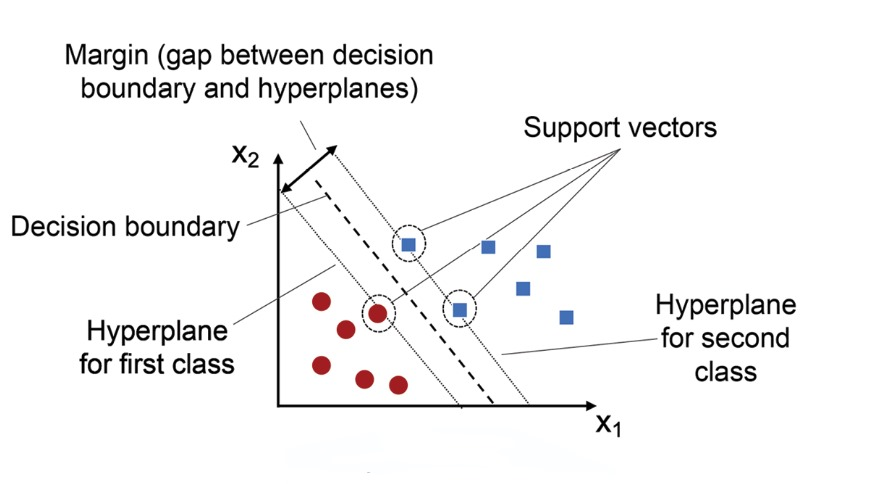
\includegraphics[width=\textwidth]{SVM.jpg}
    \caption{SVM}
    \label{fig:SVM}
\end{figure}
\\
\\
\\
\section*{SVM terminologies:-}
\begin{itemize}
\item Hyperplane: In SVM, a hyperplane is a decision boundary that separates data points of different classes in a high-dimensional space. For binary classification, it is a line in 2D space, a plane in 3D space, and a hyperplane in higher dimensions.
\item Support Vectors: These are the data points that lie closest to the hyperplane and have the most influence on its position. Support vectors are crucial in determining the optimal hyperplane and maximizing the margin.
\item Margin: The margin is the distance between the hyperplane and the nearest data points (support vectors) of each class. In SVM, the goal is to maximize this margin, as it leads to better generalization and robustness of the model.
\item Kernel Function: SVM uses kernel functions to transform data points into higher-dimensional spaces, where they can be more easily separated by a hyperplane. Common kernel functions include linear, polynomial, radial basis function (RBF), and sigmoid kernels.
\item Soft Margin: In cases where the data is not linearly separable, SVM allows for the introduction of a soft margin, which permits some misclassification errors to improve generalization. The regularization parameter C controls the trade-off between maximizing the margin and minimizing misclassification.
\item Regularization Parameter (C): This parameter in SVM controls the penalty for misclassification of data points. A smaller value of C allows for a softer margin and more misclassifications, while a larger value of C enforces a harder margin and fewer misclassifications.
\item Kernel Trick: SVM's kernel trick allows it to implicitly map data points into higher-dimensional spaces without explicitly calculating the transformed feature vectors. This makes SVM computationally efficient and enables it to handle non-linear classification tasks.
\item Decision Function: The decision function in SVM computes the distance of a data point from the hyperplane and classifies it based on its sign. If the result is positive, the point belongs to one class; if negative, it belongs to the other class.
\end{itemize}
\section*{Types of SVM}
Based on the nature of the decision boundary, Support Vector Machines (SVM) can be divided into two main parts:
\begin{enumerate}
    

\item Linear SVM: Linear SVMs use a linear decision boundary to separate the data points of different classes. When the data can be precisely linearly separated, linear SVMs are very suitable. This means that a single straight line (in 2D) or a hyperplane (in higher dimensions) can entirely divide the data points into their respective classes. A hyperplane that maximizes the margin between the classes is the decision boundary.
\newpage
\item Non-Linear SVM: Non-Linear SVM can be used to classify data when it cannot be separated into two classes by a straight line (in the case of 2D). By using kernel functions, nonlinear SVMs can handle nonlinearly separable data. The original input data is transformed by these kernel functions into a higher-dimensional feature space, where the data points can be linearly separated. A linear SVM is used to locate a nonlinear decision boundary in this modified space.
\end{enumerate}
\section{Algorithm for SVM }
\begin{enumerate}

\item Data Preparation :
The first step involves loading the stock data from a CSV file using pandas. The 'Date' column is then converted to datetime format to ensure proper sorting of the dataset in chronological order.

\item Feature Engineering :
To predict stock movements, a new column, 'Movement', is created. This column indicates whether the stock's closing price increased (1) or decreased (0) compared to the previous day. Any NaN values resulting from this calculation are removed to maintain data integrity.

\item Feature Selection :
The relevant features for the model are selected, including 'Open', 'High', 'Low', 'Close', and 'Adj Close' prices. These features are chosen based on their potential impact on stock price movements.

\item Train-Test Split :
The dataset is split into training and testing sets, with 60% of the data used for training and 40% for testing. This split ensures that the model can be evaluated on unseen data to assess its performance.

\item Data Standardization :
To prepare the data for the SVM model, the features are standardized using StandardScaler. This step ensures that all features have zero mean and unit variance, which is crucial for the SVM algorithm's performance.

\item Model Training :
An SVM classifier with a linear kernel is initialized and trained using the standardized training data. The linear kernel is chosen for its simplicity and effectiveness in binary classification tasks like this one.

\item Model Evaluation :
The trained SVM model is used to predict the stock movements on the test set. The predictions are evaluated using a confusion matrix and various performance metrics, including accuracy, precision, recall, and F1-score. These metrics provide a comprehensive understanding of the model's performance.

\item Prediction for the Next Trading Day :
The most recent data point is standardized using the same scaler. The SVM model then predicts the stock movement for the next trading day. The result is interpreted as either an increase ('Up') or a decrease ('Down') in the stock price, providing actionable insights based on the model's prediction.
\end{enumerate}
\newpage

\section{Code Snippet: (Predicting Stock Price Movement of Alibaba using SVM)}
\begin{enumerate}
        \item Importing the necessary libraries
        \begin{verbatim}
import numpy as np
import pandas as pd
from sklearn.model_selection import train_test_split
from sklearn.preprocessing import StandardScaler
from sklearn.svm import SVC
from sklearn.metrics import confusion_matrix, accuracy_score, 
precision_score, recall_score, f1_score, classification_report
       \end{verbatim}
       \item Data loading and pre processing 
       \begin{verbatim}
# Load data from a CSV file
df = pd.read_csv('baba_stock_data.csv')

# Ensure 'Date' column is in datetime format
df['Date'] = pd.to_datetime(df['Date'], format='%d-%m-%Y')

# Sorting data by date
df = df.sort_values(by='Date')

# Calculate the daily movement (1 for up, 0 for down)
df['Movement'] = (df['Close'].diff() > 0).astype(int)

# Remove the first row with NaN value due to diff()
df = df.dropna()

# Feature selection
features = ['Open', 'High', 'Low', 'Close', 'Adj Close']
X = df[features]
y = df['Movement']
     \end{verbatim}
   
     \item Model training and test split 
     \begin{verbatim}
# Train-test split
X_train, X_test, y_train, y_test =train_test_split(X,y,test_size=0.2,
random_state=0) 

# Standardize the features
scaler = StandardScaler()
X_train = scaler.fit_transform(X_train)
X_test = scaler.transform(X_test)



# Initialize and train the SVM classifier
svm_classifier = SVC(kernel='linear', random_state=0)
svm_classifier.fit(X_train, y_train)
    \end{verbatim}
    \item Predicting test results and measuring its accuracy
    \begin{verbatim}
# Predictions
y_pred = svm_classifier.predict(X_test)

# Confusion matrix
cm = confusion_matrix(y_test, y_pred)
print("Confusion Matrix:\n", cm)

# Accuracy, Precision, Recall, F1-score
accuracy = accuracy_score(y_test, y_pred)
precision = precision_score(y_test, y_pred)
recall = recall_score(y_test, y_pred)
f1 = f1_score(y_test, y_pred)

print(f'Accuracy: {accuracy:.2f}')
print(f'Precision: {precision:.2f}')
print(f'Recall: {recall:.2f}')
print(f'F1-Score: {f1:.2f}')

# Detailed classification report
print("\nClassification Report:\n", classification_report(y_test, 
y_pred))
\end{verbatim}

\item Obtaining the final results in order to predict the stock movement in the future based on the current data values :
    \begin{verbatim}
# Get the most recent data point and format it as a DataFrame
last_data_point = df[features].iloc[-1].to_frame().T

# Standardize the last data point
last_data_point_scaled = scaler.transform(last_data_point)

# Predict the movement for the next day
predicted_movement = svm_classifier.predict(last_data_point_scaled)

# Interpret the result
movement_label = "Up" if predicted_movement[0] == 1 else "Down"
print(f'The predicted movement for the next trading day is:
{movement_label}')

    \end{verbatim}
       
\end{enumerate}
\newpage
\section{Output of the code snippet-\textit{for 80:20 training:testing split}}
\begin{itemize}
    \item \underline{CONFUSION MATRIX}:
    \vspace{-0.5cm}
    \begin{flushleft}
    \[
    \begin{bmatrix}
        60 & 4 \\
        33 & 22 \\
    \end{bmatrix}
    \]
    \end{flushleft}
    \vspace{-0.5cm} % Adjust this value as needed to reduce the space between the matrix and the list items

    \item Accuracy: \textbf{0.69}
    \item Precision: \textbf{0.85}
    \item Recall: \textbf{0.40}
    \item F1-Score: \textbf{0.54}
\\
\\
    \item \underline{CLASSIFICATION REPORT}
\begin{verbatim}
                     precision    recall  f1-score   support

           0       0.65      0.94      0.76        64
           1       0.85      0.40      0.54        55

    accuracy                           0.69       119
   macro avg       0.75      0.67      0.65       119
weighted avg       0.74      0.69      0.66       119

The predicted movement for the next trading day is: Down
\end{verbatim}
\end{itemize}


\chapter{K-Nearest Neighbors (KNN)}

The k-Nearest Neighbors (k-NN) algorithm is a simple, non-parametric classification and regression technique that assigns a class or value to a data point based on the majority class or average value of its 'k' closest neighbors in the feature space. It operates on the principle that similar points are near each other and uses distance metrics like Euclidean distance to determine proximity. k-NN is easy to implement, requires no training phase, and can handle multiclass classification, but it can be computationally intensive and sensitive to irrelevant features and the choice of 'k'.
(K-NN) algorithm is a versatile and widely used machine learning algorithm that is primarily used for its simplicity and ease of implementation. It does not require any assumptions about the underlying data distribution. It can also handle both numerical and categorical data, making it a flexible choice for various types of datasets in classification and regression tasks. It is a non-parametric method that makes predictions based on the similarity of data points in a given dataset. K-NN is less sensitive to outliers compared to other algorithms.

The K-NN algorithm works by finding the K nearest neighbors to a given data point based on a distance metric, such as Euclidean distance. The class or value of the data point is then determined by the majority vote or average of the K neighbors. This approach allows the algorithm to adapt to different patterns and make predictions based on the local structure of the data.\cite{javatpoint_knn}

\begin{figure}[htbp]
    \centering
    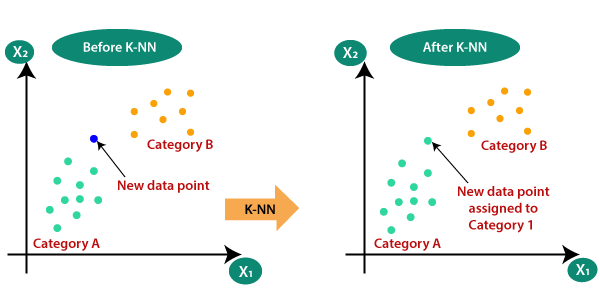
\includegraphics[width=\textwidth]{KNN.png}
    \caption{KNN}
    \label{fig:KNN}
\end{figure}

\section*{KNN terminologies:-}
\begin{itemize}
\item Training Data : The dataset used to train the k-NN model, consisting of labeled instances.
\item Instance : An individual data point in the dataset, also called a sample.
\item Feature : An individual measurable property or characteristic of a phenomenon being observed.
\item Distance Metric : A measure of similarity between instances, commonly Euclidean distance.
\item k : The number of nearest neighbors to consider for classification or regression.
\item Classification : Assigning a class label to an instance based on the majority class among its k-nearest neighbors.
\item Regression : Predicting a continuous value for an instance based on the average of the values of its k-nearest neighbors.
\item Majority Voting : In classification, the process of assigning the most frequent class label among the k-nearest neighbors.
\item Hyperparameters : Parameters such as 'k' and the distance metric that need to be set before training the model.
\item Overfitting : A model's tendency to perform well on training data but poorly on unseen data, which can occur if k is too small.
\item Underfitting : A model's inability to capture the underlying trend of the data, which can occur if k is too large.
\item Normalization : Scaling features to ensure each has a similar range, important for distance-based algorithms like k-NN.
\item Lazy Learning : k-NN is called a lazy learning algorithm because it does not build a model until a query is made.
\end{itemize}

\section{Algorithm for KNN}
\begin{codedstep}
\item Data Preparation

Begin by gathering and preparing your dataset, ensuring it includes labeled instances. Each instance should be represented by a set of features. Normalize the feature values to make sure each feature contributes equally to the distance calculations. This step is crucial as k-NN is sensitive to the scale of the data.

\item Choose the Value of k

Select an appropriate value for k, the number of nearest neighbors to consider. A small k makes the model sensitive to noise, while a large k might dilute the decision-making process. Common practice involves trying different values of k and using cross-validation to determine the optimal choice.

\item Distance Metric

Decide on a distance metric to measure similarity between instances. The Euclidean distance is most commonly used, but other metrics like Manhattan or Minkowski distances can also be applied depending on the dataset and the specific problem.

\item Find Nearest Neighbors

For each instance in the test set, calculate the distance to all instances in the training set. Identify the k instances in the training set that are closest to the test instance. These are the nearest neighbors.

\item Classification or Regression
\begin{enumerate}
\item Classification : Assign the test instance to the class that is most common among the k nearest neighbors. This is known as majority voting.
\item Regression : Predict the value for the test instance as the average (or weighted average) of the values of the k nearest neighbors.
\end{enumerate}
\item Evaluate the Model

After making predictions for the test set, evaluate the performance of the k-NN algorithm using appropriate metrics. For classification, metrics like accuracy, precision, recall, and F1-score are commonly used. For regression, you might use mean squared error or R-squared.

\item Optimization and Validation

Optimize the model by tuning the value of k and possibly the distance metric. Use techniques like cross-validation to assess the performance and ensure that the model generalizes well to unseen data. Iterate through this process to refine the model.

\item Deployment

Once satisfied with the model’s performance, deploy it for making predictions on new data. Continuously monitor its performance and update the model as necessary to adapt to new data patterns or changes in the underlying data distribution.
\end{codedstep}

\section{Code Snippet} \textit{(Predicting Stock Price Movement of Alibaba using KNN)}
\begin{enumerate}
        \item Importing the necessary libraries
        \begin{verbatim}
import numpy as np
import pandas as pd
from sklearn.model_selection import train_test_split
from sklearn.preprocessing import StandardScaler
from sklearn.svm import SVC
from sklearn.metrics import confusion_matrix, accuracy_score, 
precision_score, recall_score, f1_score, classification_report
       \end{verbatim}
       \newpage
       \item Data loading and pre-processing 
       \begin{verbatim}
# Load data from a CSV file
df = pd.read_csv('baba_stock_data.csv')

# Ensure 'Date' column is in datetime format
df['Date'] = pd.to_datetime(df['Date'], format='%d-%m-%Y')

# Sorting data by date
df = df.sort_values(by='Date')

# Calculate the daily movement (1 for up, 0 for down)
df['Movement'] = (df['Close'].diff() > 0).astype(int)

# Remove the first row with NaN value due to diff()
df = df.dropna()

# Feature selection
features = ['Open', 'High', 'Low', 'Close', 'Adj Close']
X = df[features]
y = df['Movement']

\end{verbatim}
     \item Model training and train-test split 
     \begin{verbatim}
# Train-test split
X_train, X_test, y_train, y_test = train_test_split(X, y, test_size=0.2, 
random_state=0)

# Standardize the features
scaler = StandardScaler()
X_train = scaler.fit_transform(X_train)
X_test = scaler.transform(X_test)

# Initialize and train the KNN classifier
knn = KNeighborsClassifier(n_neighbors=5)
knn.fit(X_train, y_train)
 \end{verbatim}
    \item Predicting test results and measuring its accuracy
 \begin{verbatim}
# Predictions
y_pred = knn.predict(X_test)

# Confusion matrix
cm = confusion_matrix(y_test, y_pred)
print("Confusion Matrix:\n", cm)

# Accuracy, Precision, Recall, F1-score
accuracy = accuracy_score(y_test, y_pred)
precision = precision_score(y_test, y_pred)
recall = recall_score(y_test, y_pred)
f1 = f1_score(y_test, y_pred)

print(f'Accuracy: {accuracy:.2f}')
print(f'Precision: {precision:.2f}')
print(f'Recall: {recall:.2f}')
print(f'F1-Score: {f1:.2f}')

# Detailed classification report
print("\nClassification Report:\n", classification_report(y_test, y_pred))

\end{verbatim}

\item Obtaining the final results in order to predict the stock movement in the future based on the current data values :
\begin{verbatim}

# Get the most recent data point and format it as a DataFrame
last_data_point = df[features].iloc[-1].to_frame().T

# Standardize the last data point
last_data_point_scaled = scaler.transform(last_data_point)

# Predict the movement for the next day
predicted_movement = knn.predict(last_data_point_scaled)

# Interpret the result
movement_label = "Up" if predicted_movement[0] == 1 else "Down"
print(f'The predicted movement for the next trading day is: 
{movement_label}')

\end{verbatim}
\end{enumerate}
\section{Output of the code snippet}-\textit{for 80:20 training:testing split}
\begin{itemize}
\item \underline{CONFUSION MATRIX}:
    \vspace{-0.5cm}
    \begin{flushleft}
    \[
    \begin{bmatrix}
        44 & 20 \\
        31 & 24 \\
    \end{bmatrix}
    \]
    \end{flushleft}
    \vspace{-0.5cm} % Adjust this value as needed to reduce the space between the matrix and the list items

    \item Accuracy: \textbf{0.57}
    \item Precision: \textbf{0.55}
    \item Recall: \textbf{0.44}
    \item F1-Score: \textbf{0.48}
\\
\\
    \item \underline{CLASSIFICATION REPORT}
\begin{verbatim}
               precision    recall  f1-score   support

           0       0.59      0.69      0.63        64
           1       0.55      0.44      0.48        55

    accuracy                           0.57       119
   macro avg       0.57      0.56      0.56       119
weighted avg       0.57      0.57      0.56       119

The predicted movement for the next trading day is: Up
\end{verbatim}
\end{itemize}












% Implementation
\chapter{Decision Trees (DT)}
Decision Tree is a Supervised learning technique that can be used for both classification and Regression problems, but mostly it is preferred for solving Classification problems. It is a tree-structured classifier, where internal nodes represent the features of a dataset, branches represent the decision rules and each leaf node represents the outcome.
In a Decision tree, there are two nodes, which are the Decision Node and Leaf Node. Decision nodes are used to make any decision and have multiple branches, whereas Leaf nodes are the output of those decisions and do not contain any further branches.
The decisions or the test are performed on the basis of features of the given dataset.
It is a graphical representation for getting all the possible solutions to a problem/decision based on given conditions.
It is called a decision tree because, similar to a tree, it starts with the root node, which expands on further branches and constructs a tree-like structure.
In order to build a tree, we use the CART algorithm, which stands for Classification and Regression Tree algorithm.
A decision tree simply asks a question, and based on the answer (Yes/No), it further splits the tree into subtrees. \cite{javatpoint_dt}

\begin{figure}[htbp]
    \centering
    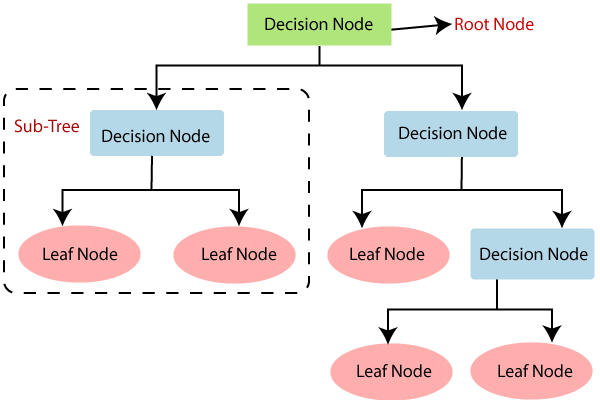
\includegraphics[width=\textwidth]{decision-tree-classification-algorithm.png}
    \caption{Decision Tree}
    \label{fig:decision-tree}
\end{figure}

\section*{Decision Tree Terminologies:-}
\begin{itemize}
\item Root Node: Root node is from where the decision tree starts. It represents the entire dataset, which further gets divided into two or more homogeneous sets.
\item Leaf Node: Leaf nodes are the final output node, and the tree cannot be segregated further after getting a leaf node.
\item Splitting: Splitting is the process of dividing the decision node/root node into sub-nodes according to the given conditions.
\item Branch/Subtree: A tree formed by splitting the tree.
\item Pruning: Pruning is the process of removing the unwanted branches from the tree.
\item Parent/Child node: The root node of the tree is called the parent node, and other nodes are called the child nodes.
\end{itemize}

\section*{Pseudo-code of the CART Algorithm (For building the decision tree)}
\begin{verbatim}
d = 0, endtree = 0
Note(0) = 1, Node(1) = 0, Node(2) = 0
while endtree < 1
   if Node(2d-1) + Node(2d) + .... + Node(2d+1-2) = 2 - 2d+1  
       endtree = 1
   else
       do i = 2d-1, 2d, .... , 2d+1-2
           if Node(i) > -1
               Split tree
           else
               Node(2i+1) = -1
               Node(2i+2) = -1
           end if
       end do
   end if
d = d + 1
end while
\end{verbatim}

\section{Working of the Decision Tree algorithm:}
In a decision tree, for predicting the class of the given dataset, the algorithm starts from the root node of the tree. This algorithm compares the values of the root attribute with the record (real dataset) attribute and, based on the comparison, follows the branch and jumps to the next node.
For the next node, the algorithm again compares the attribute value with the other sub-nodes and moves further. It continues the process until it reaches the leaf node of the tree.\newpage The complete process can be better understood using the below algorithm:
\begin{codedstep}
\item Begin the tree with the root node, says S, which contains the complete dataset.
\item Find the best attribute in the dataset using Attribute Selection Measure (ASM).
\item Divide the S into subsets that contain possible values for the best attributes.
\item Generate the decision tree node, which contains the best attribute.
\item Recursively make new decision trees using the subsets of the dataset created in step -3. Continue this process until a stage is reached where you cannot further classify the nodes and call the final node as a leaf node.
\end{codedstep}

\section*{Attribute Selection Measure (ASM)}
\begin{figure}[htbp]
    \centering
    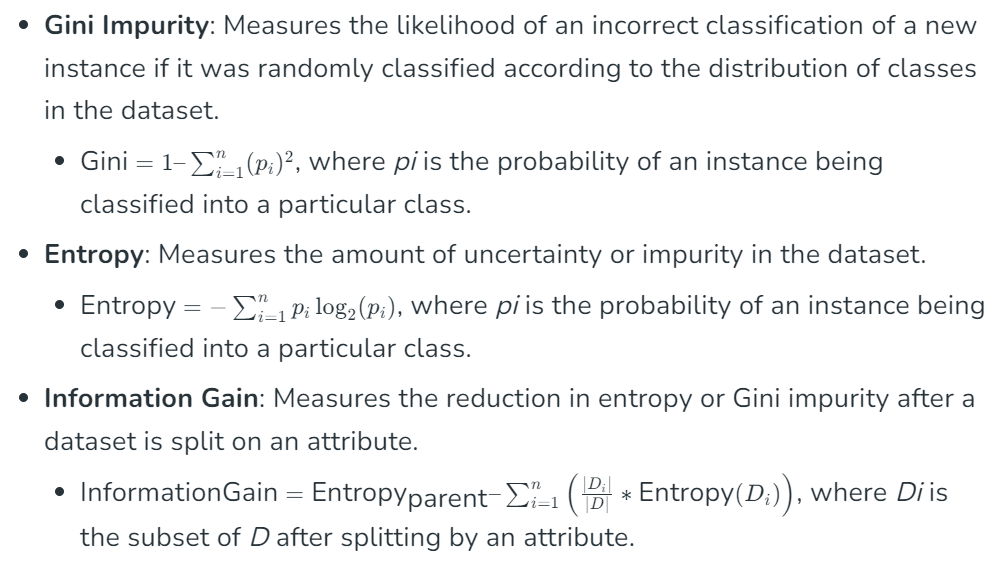
\includegraphics[width=\textwidth]{DT-2.png}
\end{figure}

The attribute with the \textbf{highest information gain} is chosen for the split. The attribute with the \textbf{largest reduction in Gini index} (or equivalently, the smallest weighted average Gini index) is chosen for the split.

\section*{Pruning: Getting an Optimal Decision tree}
Pruning is a process of deleting the unnecessary nodes from a tree in order to get the optimal decision tree.
A too-large tree increases the risk of overfitting, and a small tree may not capture all the important features of the dataset. Therefore, a technique that decreases the size of the learning tree without reducing accuracy is known as Pruning. There are mainly two types of tree pruning technology used:
\begin{enumerate}
    \item Cost Complexity Pruning
    \item Reduced Error Pruning.
\end{enumerate}

Decision trees mimic human decision-making, making them easy to understand and interpret, and are highly effective for solving sequential decision-related problems by systematically exploring all potential outcomes. They also require minimal data cleaning compared to other algorithms, handling missing values and raw data with ease.\\
\\
Decision trees can become complex with many layers and may suffer from overfitting, an issue that can be mitigated using the Random Forest algorithm. Additionally, with more class labels, the computational complexity of decision trees increases.

\section*{Common steps involved the Python Implementation of Decision Trees:-}
\begin{enumerate}
    \item Data Pre-processing step
    \item Fitting a Decision-Tree algorithm to the Training set
    \item Predicting the test result
    \item Test accuracy of the result(Creation of Confusion matrix)
    \item Visualizing the test set result.
\end{enumerate}

\section{Code Snippet} \textit{(Predicting Stock Price Movement of Alibaba using DT)}
\begin{enumerate}
    \item Importing the necessary libraries.
    \begin{verbatim}
import numpy as np
import pandas as pd
from sklearn.model_selection import train_test_split
from sklearn.tree import DecisionTreeClassifier
from sklearn.metrics import confusion_matrix, accuracy_score, 
precision_score, recall_score, f1_score, classification_report
    \end{verbatim}
    \item Data loading and pre-processing along with feature selection.
    \begin{verbatim}
# Load data from a CSV file
df = pd.read_csv('baba_stock_data.csv')

# Ensure 'Date' column is in datetime format (if not already)
df['Date'] = pd.to_datetime(df['Date'], format='%d-%m-%Y')

# Sorting data by date
df = df.sort_values(by='Date')

# Calculate the daily movement (1 for up, 0 for down)
df['Movement'] = (df['Close'].diff() > 0).astype(int)


# Remove the first row with NaN value due to diff()
df = df.dropna()

# Feature selection
features = ['Open', 'High', 'Low', 'Close', 'Adj Close']
X = df[features]
y = df['Movement']

    \end{verbatim}
    \item Model training and testing split (varying it for 4 different ratios for the result)
    \begin{verbatim}
# Train-test split for 80:20 ratio 
print("Analysis by using 80:20 split")
X_train, X_test, y_train, y_test = train_test_split(X, y, test_size=0.2, 
random_state=0)
(change test_size from 0.1 to 0.4 for different training:testing splits)
# Model training
classifier = DecisionTreeClassifier(criterion='entropy', random_state=0)
classifier.fit(X_train, y_train)

    \end{verbatim}
    \item Predicting the test results and measuring it’s accuracy:
    \begin{verbatim}
# Predictions
y_pred = classifier.predict(X_test)

# Confusion matrix
cm = confusion_matrix(y_test, y_pred)
print("Confusion Matrix:\n", cm)

# Accuracy, Precision, Recall, F1-score
accuracy = accuracy_score(y_test, y_pred)
precision = precision_score(y_test, y_pred)
recall = recall_score(y_test, y_pred)
f1 = f1_score(y_test, y_pred)

print(f'Accuracy: {accuracy:.2f}')
print(f'Precision: {precision:.2f}')
print(f'Recall: {recall:.2f}')
print(f'F1-Score: {f1:.2f}')

# Detailed classification report
print("\nClassification Report:\n", classification_report(y_test, y_pred))

    \end{verbatim}
    \newpage
    \item Obtaining the final results in order to predict the stock movement in the future based on the current data values :
    \begin{verbatim}
# Get the most recent data point and format it as a DataFrame
last_data_point = df[features].iloc[-1].to_frame().T

# Predict the movement for the next day
predicted_movement = classifier.predict(last_data_point)

# Interpret the result
movement_label = "Up" if predicted_movement[0] == 1 else "Down"
print(f'The predicted movement for the next trading day is:
{movement_label}')

    \end{verbatim}
\end{enumerate}

\section{Output of the code snippet}-\textit{for 80:20 training:testing split}
\begin{itemize}
    \item \underline{CONFUSION MATRIX}:
    \vspace{-0.5cm}
    \begin{flushleft}
    \[
    \begin{bmatrix}
        43 & 21 \\
        25 & 30 \\
    \end{bmatrix}
    \]
    \end{flushleft}
    \vspace{-0.5cm} % Adjust this value as needed to reduce the space between the matrix and the list items

    \item Accuracy: \textbf{0.61}
    \item Precision: \textbf{0.59}
    \item Recall: \textbf{0.55}
    \item F1-Score: \textbf{0.57}
\\
\\
    \item \underline{CLASSIFICATION REPORT}
\begin{verbatim}
               precision    recall  f1-score   support

           0       0.63      0.67      0.65        64
           1       0.59      0.55      0.57        55

    accuracy                           0.61       119
   macro avg       0.61      0.61      0.61       119
weighted avg       0.61      0.61      0.61       119

The predicted movement for the next trading day is: Up
\end{verbatim}
\end{itemize}

\chapter{Random Forests (RF)}
Random Forest is a popular machine learning algorithm that belongs to the supervised learning technique. It can be used for both Classification and Regression problems in ML. It is based on the concept of ensemble learning, which is a process of combining multiple classifiers to solve a complex problem and to improve the performance of the model.
As the name suggests, "Random Forest is a classifier that contains a number of decision trees on various subsets of the given dataset and takes the average to improve the predictive accuracy of that dataset." Instead of relying on one decision tree, the random forest takes the prediction from each tree and based on the majority votes of predictions, and it predicts the final output.
The greater number of trees in the forest leads to higher accuracy and prevents the problem of overfitting. \cite{javatpoint_rf}
\\
\\

\begin{figure}[htbp]
    \centering
    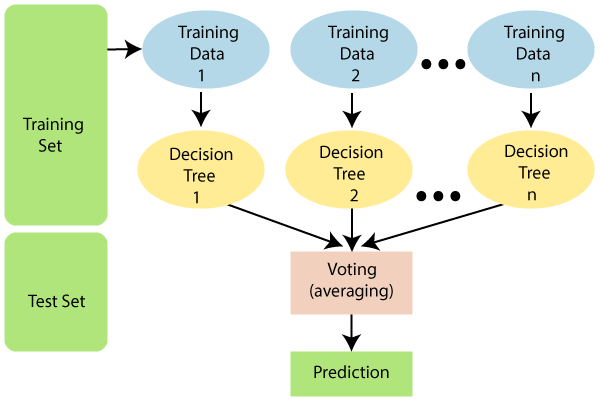
\includegraphics[width=\textwidth]{random-forest-algorithm.png}
    \caption{Random Forest}
    \label{fig:Random-forest}
\end{figure}

\newpage
Random forest is used in alternative to decision trees as:-
\begin{itemize}
    \item It takes less training time as compared to other algorithms.
    \item It predicts output with high accuracy, even for the large dataset it runs efficiently.
    \item It can also maintain accuracy when a large proportion of data is missing.
\end{itemize}
It takes less training time as compared to other algorithms.
It predicts output with high accuracy, even for the large dataset it runs efficiently.
It can also maintain accuracy when a large proportion of data is missing.

\section{Working of the Random Forest Algorithm:-}
Random Forest works in two-phase first is to create the random forest by combining N decision tree, and second is to make predictions for each tree created in the first phase.
The Working process can be explained in the below steps and diagram:
\begin{codedstep}
 \item Select random K data points from the training set. \item Build the decision trees associated with the selected data points (Subsets).
 \item Choose the number N for decision trees that you want to build.
 \item Repeat Step 1 and 2.
 \item For new data points, find the predictions of each decision tree, and assign the new data points to the category that wins the majority votes.
\end{codedstep}

The implementation is similar to that of decision trees.
\begin{itemize}
\item Data Pre-processing step
\item Fitting the Random forest algorithm to the Training set
\item Predicting the test result
\item Test accuracy of the result (Creation of Confusion matrix)
\item Visualizing the test set result.
\end{itemize}

\section{Code Snippet} \textit{(Predicting Stock Price Movement of Alibaba using RF)}
\begin{enumerate}
    \item Importing the necessary libraries.
    \begin{verbatim}
import pandas as pd
from sklearn.model_selection import train_test_split
from sklearn.ensemble import RandomForestClassifier
from sklearn.metrics import confusion_matrix, accuracy_score,
precision_score, recall_score, f1_score, classification_report
    \end{verbatim}
    \item Data loading and pre-processing along with feature selection.
    \begin{verbatim}
# Load data from a CSV file
df = pd.read_csv('baba_stock_data.csv')

# Ensure 'Date' column is in datetime format (if not already)
df['Date'] = pd.to_datetime(df['Date'], format='%d-%m-%Y')

# Sorting data by date
df = df.sort_values(by='Date')

# Calculate the daily movement (1 for up, 0 for down)
df['Movement'] = (df['Close'].diff() > 0).astype(int)

# Remove the first row with NaN value due to diff()
df = df.dropna()

# Feature selection
features = ['Open', 'High', 'Low', 'Close', 'Adj Close']
X = df[features]
y = df['Movement']
    \end{verbatim}
    \item Model training and testing split (varying it for 4 different ratios for the result)
    \begin{verbatim}
# Train-test split for 80:20
print("Analysis by using 80:20 split")
X_train, X_test, y_train, y_test = train_test_split(X, y, test_size=0.2, 
random_state=0)

# Model training
classifier = RandomForestClassifier(n_estimators=100, criterion='entropy', 
random_state=0)
classifier.fit(X_train, y_train)
    \end{verbatim}
    \item Predicting the test results and measuring it’s accuracy:
    \begin{verbatim}
# Confusion matrix
cm = confusion_matrix(y_test, y_pred)
print("Confusion Matrix:\n", cm)

# Accuracy, Precision, Recall, F1-score
accuracy = accuracy_score(y_test, y_pred)
precision = precision_score(y_test, y_pred)
recall = recall_score(y_test, y_pred)
f1 = f1_score(y_test, y_pred)

print(f'Accuracy: {accuracy:.2f}')
print(f'Precision: {precision:.2f}')
print(f'Recall: {recall:.2f}')
print(f'F1-Score: {f1:.2f}')

# Detailed classification report
print("\nClassification Report:\n", classification_report(y_test, y_pred))
    \end{verbatim}
    \item Obtaining the final results in order to predict the stock movement in the future based on the current data values :
    \begin{verbatim}
# Get the most recent data point and format it as a DataFrame
last_data_point = df[features].iloc[-1].to_frame().T

# Predict the movement for the next day
predicted_movement = classifier.predict(last_data_point)

# Interpret the result
movement_label = "Up" if predicted_movement[0] == 1 else "Down"
print(f'The predicted movement for the next trading day is:
{movement_label}')
    \end{verbatim}
\end{enumerate}

\section{Output of the code snippet}-\textit{for 80:20 training:testing split}
\begin{itemize}
    \item \underline{CONFUSION MATRIX}:
    \vspace{-0.5cm}
    \begin{flushleft}
    \[
    \begin{bmatrix}
        40 & 24 \\
        27 & 28 \\
    \end{bmatrix}
    \]
    \end{flushleft}
    \vspace{-0.5cm} % Adjust this value as needed to reduce the space between the matrix and the list items

    \item Accuracy: \textbf{0.57}
    \item Precision: \textbf{0.54}
    \item Recall: \textbf{0.51}
    \item F1-Score: \textbf{0.52}
\newpage
    \item \underline{CLASSIFICATION REPORT}
\begin{verbatim}
               precision    recall  f1-score   support

           0       0.60      0.62      0.61        64
           1       0.54      0.51      0.52        55

    accuracy                           0.57       119
   macro avg       0.57      0.57      0.57       119
weighted avg       0.57      0.57      0.57       119

The predicted movement for the next trading day is: Up
\end{verbatim}
\end{itemize}


\chapter{Artificial Neural Networks (ANN)}
An Artificial Neural Network (ANN) is a sophisticated machine learning algorithm inspired by the human brain's neural networks, designed for pattern recognition and learning from data. It consists of interconnected processing units called neurons, organized into three types of layers: the input layer, which receives the initial data; one or more hidden layers, which perform intermediate computations and feature extraction; and the output layer, which produces the final predictions. Each neuron receives inputs weighted by their importance, processes them, and passes the result through an activation function, which introduces non-linearity and enables the network to model complex relationships. The network learns by adjusting these weights and biases during training to minimize the error in predictions through a method called back propagation. This process allows ANNs to excel in various applications, including image and speech recognition, natural language processing, and predictive analytics, making them a versatile tool for solving complex real-world problems. \cite{geeksforgeeks_ann}

\begin{figure}[htbp]
    \centering
    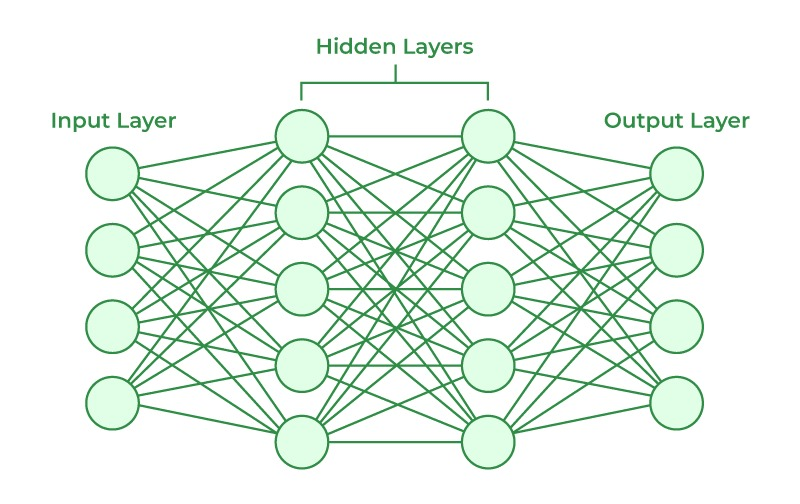
\includegraphics[width=\textwidth]{ANN_ALOGORITHM.jpg}
    \caption{Artificial Neural Networks}
    \label{fig:ANN}
\end{figure}

\section*{Artificial Neural Networks Terminologies:-}
\begin{itemize}
\item Neuron (Node): The basic computational unit of an ANN, representing a mathematical function that receives one or more inputs, applies weights to them, and produces an output using an activation function.
\item Input Layer: The first layer of the ANN that receives the initial input data and passes it to the subsequent layers for processing.
\item Hidden Layer: Intermediate layers between the input and output layers where the processing of data occurs. These layers help in feature extraction and transformation.
\item Output Layer: The final layer of the ANN that produces the network's output, usually in the form of predictions or classifications.
\item Weights: Parameters associated with the connections between neurons, representing the strength of the connection. They are adjusted during training to minimize the error in predictions.
\item Biases: Additional parameters added to neurons that allow the network to learn the offset from zero.
\item Activation Function: A mathematical function applied to the weighted sum of inputs in a neuron to introduce non-linearity and determine the neuron's output. Common activation functions include sigmoid, tanh, ReLU (Rectified Linear Unit), and softmax.
\item Feedforward: The process of passing input data through the network to produce an output without any feedback loop.
\item Backpropagation: A training algorithm used to update the weights of the network based on the difference between predicted and actual outputs. It involves calculating gradients of the loss function with respect to each weight and adjusting them to minimize the error.
\item Loss Function: A function that measures the difference between predicted and actual outputs, quantifying the performance of the network during training.
\item Optimization Algorithm: A method used to minimize the loss function and update the weights during training. Common optimization algorithms include Gradient Descent, Stochastic Gradient Descent (SGD), Adam, and RMSprop.
\item Epoch: One complete pass through the entire training dataset during the training process.
\item Batch Size: The number of training examples used in one iteration of training.
\item Learning Rate: A hyperparameter that determines the step size of weight updates during training, influencing the convergence and stability of the training process.
\end{itemize}
\newpage
\section{Algorithm for Artificial Neural Networks}
\begin{codedstep}
\item Initialize the network,
Initialize the weights and biases randomly.
Choose the number of layers and neurons in each layer.
Choose the activation function for each neuron.
\item Forward Propagation.\\
For each training example :
    Set the input values for the input layer. 
    For each hidden layer and output layer and follow these:-\\
            - Calculate the weighted sum of inputs (z) for each neuron\\
            - Apply the activation function to compute the output of each neuron
\item Calculate Loss -
Compute the loss function to measure the difference between predicted and actual outputs
\item Backpropagation.\\
For each training example:
    Compute the gradient of the loss function with respect to each weight and bias using the chain rule. Update the weights and biases using an optimization algorithm (e.g., Gradient Descent):\\
        - NewWeight = OldWeight - LearningRate * Gradient
\item Repeat Steps 2-4 :
Repeat for a fixed number of epochs or until convergence criteria are met
\item Prediction\\
For a new input:
    - Perform forward propagation to obtain the predicted output
\item Evaluation:
Compute evaluation metrics (e.g., accuracy, precision, recall, F1-score) using the predicted outputs and true labels
\item Repeat Steps 1-7 :
Repeat with different network architectures, hyperparameters, and optimization algorithms to improve performance
\end{codedstep}

\section*{Pseudo Code for Artificial neural networks}
\begin{verbatim}
Step 1: Initialize the network
def initialize_network():
    network = []
    num_layers = 3  # Number of layers including input,hidden,and output layers
    input_layer_size = 10  # Number of neurons in the input layer
    hidden_layer_size = 8  # Number of neurons in the hidden layer
    output_layer_size = 1  # Number of neurons in the output layer
    
    Initialize weights and biases for each layer randomly
    for i in range(num_layers - 1):
        if i == 0:
            weights =random_initialization(input_layer_size, hidden_layer_size)
        elif i == num_layers - 2:
            weights =random_initialization(hidden_layer_size, output_layer_size)
        else:
            weights =random_initialization(hidden_layer_size, hidden_layer_size)
        biases = random_initialization(1, hidden_layer_size)
        network.append({'weights': weights, 'biases': biases})
    return network

def random_initialization(rows, cols):
    return np.random.randn(rows, cols)

Step 2: Forward Propagation
def forward_propagation(network, inputs):
    layer_outputs = inputs
    for layer in network:
        weighted_sum = np.dot(layer_outputs, layer['weights']) + layer['biases']
        layer_outputs = activation_function(weighted_sum)
    return layer_outputs

Step 3: Loss Calculation
def calculate_loss(predicted_output, actual_output):
    loss = 0.5 * ((predicted_output - actual_output) ** 2)  
    return loss

Step 4: Backpropagation
def backpropagation(network, inputs, target_output, learning_rate):
    outputs = []
    layer_outputs = inputs
    for layer in network:
        weighted_sum = np.dot(layer_outputs, layer['weights']) + layer['biases']
        layer_outputs = activation_function(weighted_sum)
        outputs.append(layer_outputs)
    
    errors = [target_output - outputs[-1]]
    for i in range(len(network) - 1, 0, -1):
        error = np.dot(errors[-1], network[i]['weights'].T)
        errors.append(error)
    
    for i in range(len(network)):
        network[i]['weights'] += learning_rate * np.dot(inputs.T, 
        errors[len(network) - i - 1])
        network[i]['biases'] += learning_rate * 
        np.sum(errors[len(network) - i - 1], axis=0, keepdims=True)

Step 5: Training Loop
def train_network(network, train_inputs, train_targets, epochs, learning_rate):
    for epoch in range(epochs):
        total_loss = 0
        for inputs, target_output in zip(train_inputs, train_targets):
            outputs = forward_propagation(network, inputs)
            loss = calculate_loss(outputs, target_output)
            total_loss += loss
            backpropagation(network, inputs, target_output, learning_rate)
        average_loss = total_loss / len(train_inputs)
        print(f'Epoch {epoch + 1}, Loss: {average_loss}')

Step 6: Prediction
def predict(network, test_inputs):
    predictions = []
    for inputs in test_inputs:
        outputs = forward_propagation(network, inputs)
        predictions.append(outputs)
    return predictions

Step 7: Evaluation
def evaluate(predictions, actual_outputs):
    Compute evaluation metrics (e.g., accuracy, precision, recall, F1-score)
    pass

Step 8: Main Function
def main():
    Example usage
    network = initialize_network()
    train_network(network,train_inputs,train_targets,epochs=100
    ,learning_rate=0.01)
    test_predictions = predict(network, test_inputs)
    evaluation = evaluate(test_predictions, test_targets)

if _name_ == "_main_":
    main()
\end{verbatim}
\section{Code Snippet} \textit{(Predicting Stock Price Movement of Alibaba using ANN)}
\begin{enumerate}
        \item Importing the necessary libraries
        \begin{verbatim}
import numpy as np
import pandas as pd
from sklearn.model_selection import train_test_split
from sklearn.preprocessing import StandardScaler
from sklearn.metrics import confusion_matrix, accuracy_score, 
precision_score, recall_score, f1_score, classification_report
from tensorflow.keras.models import Sequential
from tensorflow.keras.layers import Dense
       \end{verbatim}
       \item Data loading and pre-processing 
       \begin{verbatim}
# Load data from a CSV file
df = pd.read_csv('baba_stock_data.csv')

# Ensure 'Date' column is in datetime format
df['Date'] = pd.to_datetime(df['Date'], format='%Y-%m-%d')

# Sorting data by date
df = df.sort_values(by='Date')

# Calculate the daily movement (1 for up, 0 for down)
df['Movement'] = (df['Close'].diff() > 0).astype(int)

# Remove the first row with NaN value due to diff()
df = df.dropna()

# Feature selection
features = ['Open', 'High', 'Low', 'Close', 'Adj Close']
X = df[features]
y = df['Movement']
     \end{verbatim}
     \item Model training and train-test split 
     \begin{verbatim}
 # Train-test split
X_train, X_test, y_train, y_test = train_test_split(X, y, test_size=0.2,
random_state=0)

# Standardize the features
scaler = StandardScaler()
X_train = scaler.fit_transform(X_train)
X_test = scaler.transform(X_test)

# Initialize the ANN
model = Sequential()
model.add(Dense(units=64, activation='relu', input_dim=X_train.shape[1]))
model.add(Dense(units=32, activation='relu'))
model.add(Dense(units=1, activation='sigmoid'))

# Compile the ANN
model.compile(optimizer='adam', loss='binary_crossentropy', 
metrics=['accuracy'])

# Train the ANN
model.fit(X_train, y_train, epochs=50, batch_size=10, verbose=1)
       \end{verbatim}
       \item Predicting results and measuring accuracy
       \begin{verbatim}
# Predictions
y_pred = model.predict(X_test)
y_pred = (y_pred > 0.5).astype(int)

# Confusion matrix
cm = confusion_matrix(y_test, y_pred)
print("Confusion Matrix:\n", cm)

# Accuracy, Precision, Recall, F1-score
accuracy = accuracy_score(y_test, y_pred)
precision = precision_score(y_test, y_pred)
recall = recall_score(y_test, y_pred)
f1 = f1_score(y_test, y_pred)

print(f'Accuracy: {accuracy:.2f}')
print(f'Precision: {precision:.2f}')
print(f'Recall: {recall:.2f}')
print(f'F1-Score: {f1:.2f}')

# Detailed classification report
print("\nClassification Report:\n", classification_report(y_test, y_pred))

# Get the most recent data point and format it as a DataFrame
last_data_point = df[features].iloc[-1].to_frame().T

# Standardize the last data point
last_data_point_scaled = scaler.transform(last_data_point)

# Predict the movement for the next day
predicted_movement = model.predict(last_data_point_scaled)
predicted_movement = (predicted_movement > 0.5).astype(int)

# Interpret the result
movement_label = "Up" if predicted_movement[0][0] == 1 else "Down"
print(f'The predicted movement for the next trading day is:
{movement_label}')
       \end{verbatim}
\end{enumerate}
\section{Output of the code snippet}-\textit{for 80:20 training:testing split}
\begin{itemize}
    \item \underline{CONFUSION MATRIX}:
    \vspace{-0.5cm}
    \begin{flushleft}
    \[
    \begin{bmatrix}
        52 & 12 \\
        18 & 37 \\
    \end{bmatrix}
    \]
    \end{flushleft}
    \vspace{-0.5cm}

    \item Accuracy: \textbf{0.75}
    \item Precision: \textbf{0.76}
    \item Recall: \textbf{0.67}
    \item F1-Score: \textbf{0.71}
\newpage
    \item \underline{CLASSIFICATION REPORT}
\begin{verbatim}
                  precision    recall  f1-score   support

           0       0.74      0.81      0.78        64
           1       0.76      0.67      0.71        55

    accuracy                           0.75       119
   macro avg       0.75      0.74      0.74       119
weighted avg       0.75      0.75      0.75       119

The predicted movement for the next trading day is: Up
\end{verbatim}
\end{itemize}






\chapter{Reinforcement Learning (RL)}
\vspace{-1cm}
Reinforcement Learning is a feedback-based Machine learning technique in which an agent learns to behave in an environment by performing the actions and seeing the results of actions. For each good action, the agent gets positive feedback, and for each bad action, the agent gets negative feedback or penalty.
In Reinforcement Learning, the agent learns automatically using feedbacks without any labeled data, unlike supervised learning.
Since there is no labeled data, so the agent is bound to learn by its experience only.
RL solves a specific type of problem where decision making is sequential, and the goal is long-term, such as game-playing, robotics, etc.
The agent interacts with the environment and explores it by itself. The primary goal of an agent in reinforcement learning is to improve the performance by getting the maximum positive rewards.
The agent learns with the process of hit and trial, and based on the experience, it learns to perform the task in a better way. Hence, we can say that "Reinforcement learning is a type of machine learning method where an intelligent agent (computer program) interacts with the environment and learns to act within that." How a Robotic dog learns the movement of his arms is an example of Reinforcement learning.
It is a core part of Artificial intelligence, and all AI agent works on the concept of reinforcement learning. Here we do not need to pre-program the agent, as it learns from its own experience without any human intervention.
Example: Suppose there is an AI agent present within a maze environment, and his goal is to find the diamond. The agent interacts with the environment by performing some actions, and based on those actions, the state of the agent gets changed, and it also receives a reward or penalty as feedback.
The agent continues doing these three things (take action, change state/remain in the same state, and get feedback), and by doing these actions, he learns and explores the environment.
The agent learns that what actions lead to positive feedback or rewards and what actions lead to negative feedback penalty. As a positive reward, the agent gets a positive point, and as a penalty, it gets a negative point. \cite{javatpoint_rl}

\section*{Key Features of Reinforcement Learning}
\begin{enumerate}
\item In RL, the agent is not instructed about the environment and what actions need to be taken.
\item It is based on the hit and trial process.
\item The agent takes the next action and changes states according to the feedback of the previous action.
\item The agent may get a delayed reward.
\item The environment is stochastic, and the agent needs to explore it to reach to get the maximum positive rewards.
\end{enumerate}
\begin{figure}[htbp]
    \centering
    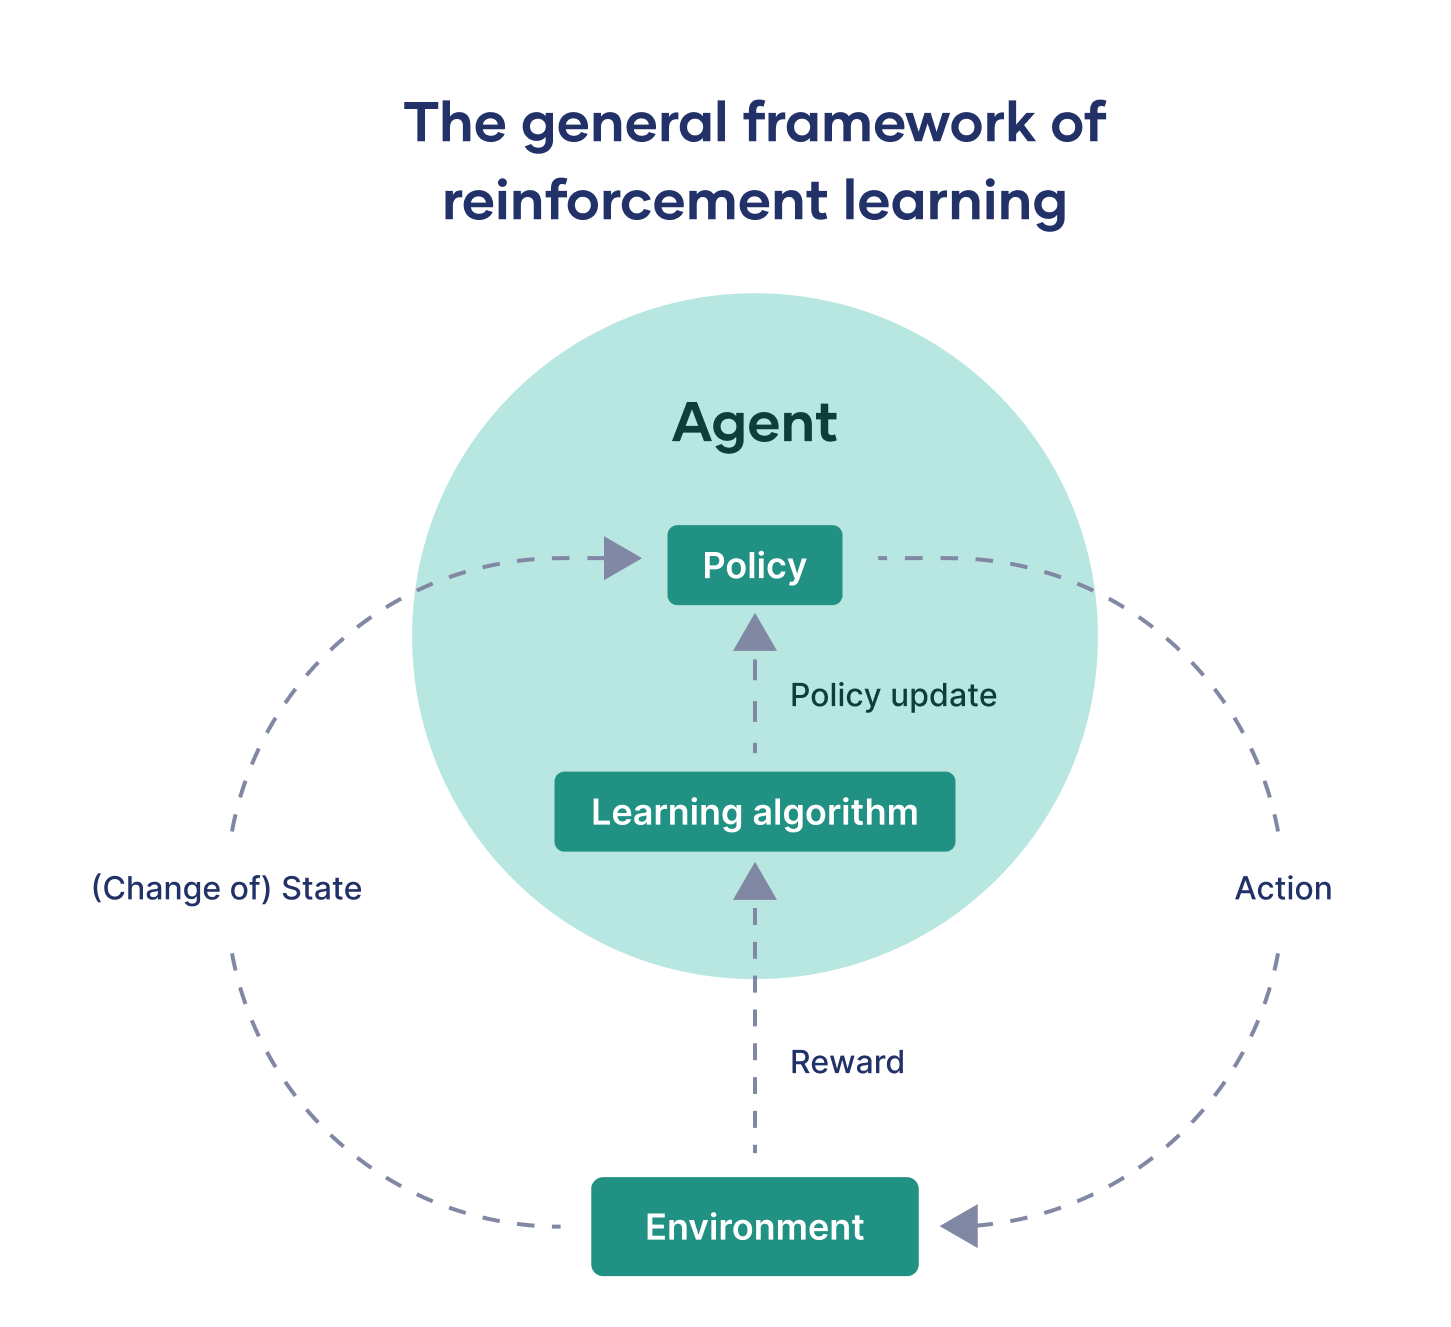
\includegraphics[width=\textwidth]{the-general-framework-of-reinforcement-learning.png}
    \caption{Reinforcement Learning}
    \label{fig:Reinforcement Learning}
\end{figure}

\section*{Terms used in Reinforcement Learning}
\begin{itemize}
    \item Agent(): An entity that can perceive/explore the environment and act upon it.
    \item Environment(): A situation in which an agent is present or surrounded by. In RL, we assume the stochastic environment, which means it is random in nature.
    \item Action(): Actions are the moves taken by an agent within the environment.
    \item State(): State is a situation returned by the environment after each action taken by the agent.
    \item Reward(): A feedback returned to the agent from the environment to evaluate the action of the agent.
    \item Policy(): Policy is a strategy applied by the agent for the next action based on the current state.
    \item Value(): It is expected long-term retuned with the discount factor and opposite to the short-term reward.
    \item Q-value(): It is mostly similar to the value, but it takes one additional parameter as a current action (a).

\end{itemize}

\section*{Elements of Reinforcement Learning}
Reinforcement learning elements are as follows:
\begin{enumerate}
    \item Policy
    \item Reward function
    \item Value function
    \item Model of the environment
\end{enumerate}

Policy: Policy defines the learning agent behavior for given time period. It is a mapping from perceived states of the environment to actions to be taken when in those states.

Reward function: Reward function is used to define a goal in a reinforcement learning problem.A reward function is a function that provides a numerical score based on the state of the environment

Value function: Value functions specify what is good in the long run. The value of a state is the total amount of reward an agent can expect to accumulate over the future, starting from that state.

Model of the environment: Models are used for planning.

\section*{Approaches to implement Reinforcement Learning}
There are mainly three ways to implement reinforcement-learning in ML, which are:
\begin{enumerate}
\item Value-based:
The value-based approach is about to find the optimal value function, which is the maximum value at a state under any policy. Therefore, the agent expects the long-term return at any state(s) under policy π.
\item Policy-based:
Policy-based approach is to find the optimal policy for the maximum future rewards without using the value function. In this approach, the agent tries to apply such a policy that the action performed in each step helps to maximize the future reward.\\
The policy-based approach has mainly two types of policy:
\begin{enumerate}
\item Deterministic: The same action is produced by the policy (π) at any state.
\item Stochastic: In this policy, probability determines the produced action.
\end{enumerate}
\item Model-based: In the model-based approach, a virtual model is created for the environment, and the agent explores that environment to learn it. There is no particular solution or algorithm for this approach because the model representation is different for each environment.
\end{enumerate}

\section*{Types of Reinforcement:} 

There are two types of Reinforcement:  
\begin{enumerate}

    \item Positive: Positive Reinforcement is defined as when an event, occurs due to a particular behavior, increases the strength and the frequency of the behavior. In other words, it has a positive effect on behavior.
\begin{itemize}
\renewcommand\labelitemi{--}
\item Maximizes Performance
\item Sustain Change for a long period of time
\item Too much Reinforcement can lead to an overload of states which can diminish the results\\
\end{itemize}
\item Negative: Negative Reinforcement is defined as strengthening of behavior because a negative condition is stopped or avoided. 
\begin{itemize}
\renewcommand\labelitemi{--}
\item Increases Behavior
\item Provide defiance to a minimum standard of performance
\item It Only provides enough to meet up the minimum behavior
\end{itemize}
\end{enumerate}
\vspace{1cm}
 \textbf{Markov Decision Process or MDP}, is used to formalize the reinforcement learning problems. If the environment is completely observable, then its dynamic can be modeled as a Markov Process. In MDP, the agent constantly interacts with the environment and performs actions; at each action, the environment responds and generates a new state.MDP is used to describe the environment for the RL, and almost all the RL problem can be formalized using MDP.

MDP contains a tuple of four elements (S, A, Pa, Ra):
\begin{itemize}
\item A set of finite States S
\item A set of finite Actions A
\item Rewards received after transitioning from state S to state S', due to action a.
\item Probability Pa.
\end{itemize}
MDP uses the Markov property as described below:\\

\textbf{Markov Property:}
It says that "If the agent is present in the current state s1, performs an action a1 and move to the state s2, then the state transition from s1 to s2 only depends on the current state and future action and states do not depend on past actions, rewards, or states."
\\ \\
Or, in other words, as per the Markov Property, the current state transition does not depend on any past action or state. Hence, MDP is an RL problem that satisfies the Markov property. Such as in a Chess game, the players only focus on the current state and do not need to remember past actions or states.
\\ \\
\textit{Finite MDP:}

A finite MDP is when there are finite states, finite rewards, and finite actions. In RL, we consider only the finite MDP.
\\ \\
\textbf{Markov Process:}
Markov Process is a memoryless process with a sequence of random states S1, S2, ....., St that uses the Markov Property. Markov process is also known as Markov chain, which is a tuple (S, P) on state S and transition function P. These two components (S and P) can define the dynamics of the system.

In this report , we are using the reinforcement algorithm of \textbf{Q-Learning}.

\section{Reinforcement Algorithm: Q-Learning}

Q-learning is an Off policy RL algorithm, which is used for the temporal difference Learning. The temporal difference learning methods are the way of comparing temporally successive predictions.
It learns the value function Q (S, a), which means how good to take action "a" at a particular state "s."
% \vspace{-1cm}
\begin{figure}[h!]
    \centering
    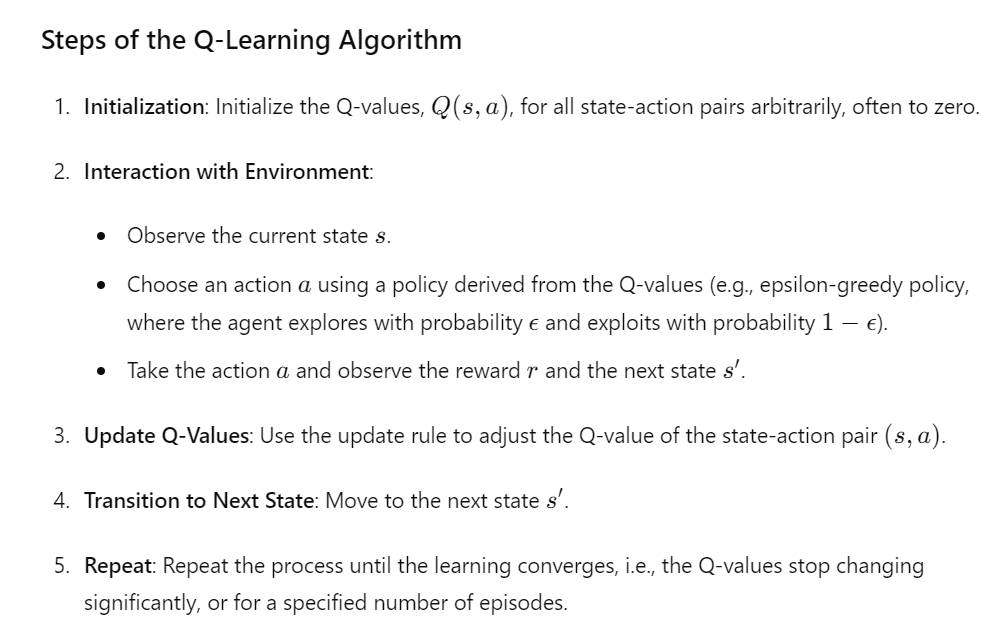
\includegraphics[width=\textwidth]{RL-1.png}
    \caption{Reinforcement Learning}
    \label{fig:Reinforcement Learning}
\end{figure}
\begin{figure}[htbp]
    \centering
    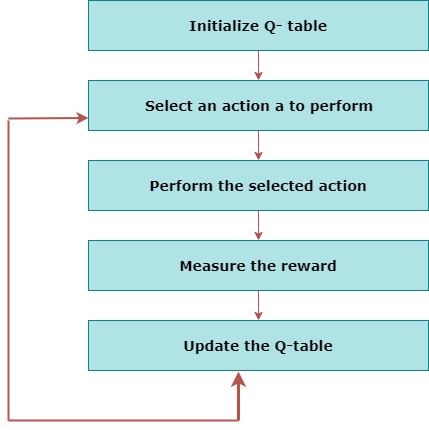
\includegraphics[width=\textwidth]{reinforcement-learning-algorithms.png}
    \caption{Q Learning Algorithm}
    \label{fig:Q-Learning}
\end{figure}
\newpage
\section{Code Snippet} \textit{(Predicting Stock Price Movement of Alibaba using Reinforcement Learning)}


\begin{enumerate}
        \item Importing the Necessary Libraries
        \begin{verbatim}
import numpy as np
import pandas as pd
from sklearn.model_selection import train_test_split
from sklearn.preprocessing import StandardScaler
from sklearn.metrics import confusion_matrix, precision_score, 
accuracy_score, recall_score, f1_score
import random
# Seed for reproducibility
random.seed(42)
       \end{verbatim}
       \item Data Loading and Pre-processing 
       \begin{verbatim}
# Loading our stock dataset
file_path = 'baba_stock_data.csv'
data = pd.read_csv(file_path)

# Convert Date to datetime to sort by date
data['Date'] = pd.to_datetime(data['Date'])
data = data.sort_values('Date')

# Feature engineering - creating a new target variable 
`Profitable` (0/1) based on if the stock price increased or 
decreased on that day
data['Profitable'] = (data['Close'] > data['Open']).astype(int)

# Select relevant features (excluding 'Adj Close')
X = data[['Open', 'High', 'Low', 'Close', 'Volume']]
y = data['Profitable']
dates = data['Date']
       \end{verbatim}
     \item Model Training and Train-test Split 
     \begin{verbatim}
# 80:20 training-testing ratio
ratio = 0.2

# Split the dataset
X_train, X_test, y_train, y_test, dates_train, dates_test = 
train_test_split(X, y, dates, test_size=ratio, random_state=42)

# Standardize the features
scaler = StandardScaler()
X_train = scaler.fit_transform(X_train)
X_test = scaler.transform(X_test)
# Reinforcement Learning (Q-learning)
def q_learning_train(X, y, episodes=1000,
learning_rate=0.1, discount_factor=0.95, epsilon=0.1):
    n_actions = 2  # Buy or Sell (0 or 1)
    n_states = X.shape[0]
    
    # Initialize Q-table with zeros
    Q = np.zeros((n_states, n_actions))
    
    for _ in range(episodes):
        state = random.randint(0, n_states - 1)
        while True:
            if random.uniform(0, 1) < epsilon:
            # epsilon is our exploration rate
                action = random.randint(0, n_actions - 1)  # Explore
            else:
                action = np.argmax(Q[state, :])  # Exploit
            
            reward = y.iloc[state] if action == 1 else -y.iloc[state]
            
            next_state = (state + 1) % n_states
            Q[state, action] = Q[state, action] + 
             learning_rate * (reward + discount_factor * 
        np.max(Q[next_state, :]) - Q[state, action])
            
            state = next_state
            if state == 0:
                break
    
    return Q

# Train Q-learning model
Q = q_learning_train(pd.DataFrame(X_train), y_train)
\end{verbatim}
       \item Predicting Results and Measuring Accuracy
       \begin{verbatim}
def q_learning_predict(Q, X):
    '''Predicts the actions for each state in X (test data) 
    using the Q-table.'''
    y_pred = []
    for state in range(X.shape[0]):
        action = np.argmax(Q[state, :])
        y_pred.append(action)
    return np.array(y_pred)

y_pred_q = q_learning_predict(Q, pd.DataFrame(X_test))

def print_confusion_matrix(cm, title):
    print(f"{title} Confusion Matrix:")
    print(cm,end='\n\n')

# Calculate metrics
precision_q = precision_score(y_test, y_pred_q)
accuracy_q = accuracy_score(y_test, y_pred_q)
recall_q = recall_score(y_test, y_pred_q)
f1_q = f1_score(y_test, y_pred_q)

# Display results
print("\nResults for 80:20 Training-Testing Ratio:")
print_confusion_matrix(confusion_matrix(y_test, y_pred_q), "Q-
learning")
print(f"Precision: {precision_q}")
print(f"Accuracy: {accuracy_q}")
print(f"Recall: {recall_q}")
print(f"F1 Score: {f1_q}")
       \end{verbatim}
\end{enumerate}




\section{Output of the code snippet}\textit{for 80:20 training:testing split}

\begin{itemize}
    \item \underline{Confusion Matrix}:
    \vspace{-0.5cm}
    \begin{flushleft}
    \[
    \begin{bmatrix}
        20 & 29 \\
        27 & 43 \\
    \end{bmatrix}
    \]
    \end{flushleft}
    \vspace{-0.5cm}
    \item Accuracy: \textbf{0.529}
    \item Precision: \textbf{0.597}
    \item Recall: \textbf{0.614}
    \item F1-Score: \textbf{0.605}
\end{itemize}

Here we predict the profitable days (1 for profitable and 0 for not profitable) using Reinforcement Learning Algorithm.

\chapter{Results and Discussion}
\vspace{-1cm}
\begin{figure}[h]
    \centering
    \begin{minipage}{\textwidth}
        \centering
        \captionof{table}{Precision Table}
        \begin{tabular}{ |c|c|c|c|c|c|c| } 
            \hline
            Ratio & SVM & KNN & RF & DT & ANN & Reinforcement \\
            \hline
            60:40 & 0.83 & 0.62 & 0.65 & 0.63 & 0.72 & 0.53\\
            70:30 & 0.84 & 0.58 & 0.63 & 0.61 & 0.77 & 0.53\\
            80:20 & 0.85 & 0.55 & 0.54 & 0.59 & 0.76 & 0.56\\
            90:10 & 0.84 & 0.71 & 0.77 & 0.73 & 0.77 & 0.72\\
            \hline
            Avg & 0.84 & 0.61 & 0.64 & 0.64 & 0.75 & 0.59\\
            \hline
        \end{tabular}
    \end{minipage}
    
    \vspace{1cm}
    
    \begin{minipage}{\textwidth}
        \centering
        \begin{tikzpicture}
            \begin{axis}[
                ybar,
                bar width=.5cm,
                width=.7\textwidth,
                height=.5\textwidth,
                enlarge x limits=0.3,
                xlabel={Algorithm},
                ylabel={Precision},
                symbolic x coords={SVM, KNN, RF, DT, ANN, Reinforcement},
                xtick=data,
                nodes near coords,
                ymin=0,
                ymax=1,
                xticklabel style={anchor=east, rotate=45}
                ]
                \addplot coordinates {(SVM,0.84) (KNN,0.61) (RF,0.64) (DT,0.64) (ANN,0.75) (Reinforcement,0.59)};
            \end{axis}
        \end{tikzpicture}
        \caption{Average Precision for Different Algorithms}
        \label{fig:precision}
    \end{minipage}
\end{figure}

\begin{figure}[h]
    \centering
    \begin{minipage}{\textwidth}
        \centering
        \captionof{table}{Accuracy Table}
        \begin{tabular}{ |c|c|c|c|c|c|c| } 
            \hline
            Ratio & SVM & KNN & RF & DT & ANN & Reinforcement\\
            \hline
            60:40 & 0.61 & 0.58 & 0.61 & 0.61 & 0.72 & 0.45\\
            70:30 & 0.62 & 0.57 & 0.61 & 0.60 & 0.70 & 0.51\\
            80:20 & 0.69 & 0.57 & 0.57 & 0.61 & 0.75 & 0.49\\
            90:10 & 0.72 & 0.65 & 0.70 & 0.70 & 0.78 & 0.63\\
            \hline
            Avg & 0.66 & 0.59 & 0.62 & 0.63 & 0.73 & 0.52\\
            \hline
        \end{tabular}
    \end{minipage}
    
    \vspace{1cm}
    
    \begin{minipage}{\textwidth}
        \centering
        \begin{tikzpicture}
            \begin{axis}[
                ybar,
                bar width=.5cm,
                width=.7\textwidth,
                height=.5\textwidth,
                enlarge x limits=0.3,
                xlabel={Algorithm},
                ylabel={Accuracy},
                symbolic x coords={SVM, KNN, RF, DT, ANN, Reinforcement},
                xtick=data,
                nodes near coords,
                ymin=0,
                ymax=1,
                xticklabel style={anchor=east, rotate=45}
                ]
                \addplot coordinates {(SVM,0.66) (KNN,0.59) (RF,0.62) (DT,0.63) (ANN,0.73) (Reinforcement,0.52)};
            \end{axis}
        \end{tikzpicture}
        \caption{Average Accuracy for Different Algorithms}
        \label{fig:accuracy}
    \end{minipage}
\end{figure}

\begin{figure}[h]
    \centering
    \begin{minipage}{\textwidth}
        \centering
        \captionof{table}{Recall Table}
        \begin{tabular}{ |c|c|c|c|c|c|c| } 
            \hline
            Ratio & SVM & KNN & RF & DT & ANN & Reinforcement \\
            \hline
            60:40 & 0.29 & 0.45 & 0.50 & 0.55 & 0.73 & 0.49\\
            70:30 & 0.30 & 0.49 & 0.53 & 0.52 & 0.55 & 0.60\\
            80:20 & 0.40 & 0.44 & 0.51 & 0.55 & 0.67 & 0.60\\
            90:10 & 0.53 & 0.50 & 0.57 & 0.63 & 0.80 & 0.69\\
            \hline
            Avg & 0.38 & 0.47 & 0.52 & 0.56 & 0.68 & 0.59\\
            \hline
        \end{tabular}
    \end{minipage}
    
    \vspace{1cm}
    
    \begin{minipage}{\textwidth}
        \centering
        \begin{tikzpicture}
            \begin{axis}[
                ybar,
                bar width=.5cm,
                width=.7\textwidth,
                height=.5\textwidth,
                enlarge x limits=0.3,
                xlabel={Algorithm},
                ylabel={Recall},
                symbolic x coords={SVM, KNN, RF, DT, ANN, Reinforcement},
                xtick=data,
                nodes near coords,
                ymin=0,
                ymax=1,
                xticklabel style={anchor=east, rotate=45}
                ]
                \addplot coordinates {(SVM,0.38) (KNN,0.47) (RF,0.52) (DT,0.56) (ANN,0.68) (Reinforcement,0.59)};
            \end{axis}
        \end{tikzpicture}
        \caption{Average Recall for Different Algorithms}
        \label{fig:recall}
    \end{minipage}
\end{figure}

\begin{figure}[h]
    \centering
    \begin{minipage}{\textwidth}
        \centering
        \captionof{table}{Score Table}
        \begin{tabular}{ |c|c|c|c|c|c|c| } 
            \hline
            Ratio & SVM & KNN & RF & DT & ANN & Reinforcement \\
            \hline
            60:40 & 0.43 & 0.52 & 0.57 & 0.59 & 0.72 & 0.51\\
            70:30 & 0.44 & 0.53 & 0.58 & 0.56 & 0.64 & 0.58\\
            80:20 & 0.54 & 0.48 & 0.65 & 0.57 & 0.71 & 0.58\\
            90:10 & 0.65 & 0.59 & 0.65 & 0.68 & 0.79 & 0.71\\
            \hline
            Avg & 0.51 & 0.53 & 0.61 & 0.60 & 0.71 & 0.59\\
            \hline
        \end{tabular}
    \end{minipage}
    
    \vspace{1cm}
    
    \begin{minipage}{\textwidth}
        \centering
        \begin{tikzpicture}
            \begin{axis}[
                ybar,
                bar width=.5cm,
                width=.7\textwidth,
                height=.5\textwidth,
                enlarge x limits=0.3,
                xlabel={Algorithm},
                ylabel={F1-Score},
                symbolic x coords={SVM, KNN, RF, DT, ANN, Reinforcement},
                xtick=data,
                nodes near coords,
                ymin=0,
                ymax=1,
                xticklabel style={anchor=east, rotate=45}
                ]
                \addplot coordinates {(SVM,0.51) (KNN,0.53) (RF,0.61) (DT,0.60) (ANN,0.71) (Reinforcement,0.59)};
            \end{axis}
        \end{tikzpicture}
        \caption{Average F1-Score for Different Algorithms}
        \label{fig:f1score}
    \end{minipage}
\end{figure}


\chapter{Conclusion}

This report comprehensively evaluates six prominent machine learning algorithms—Support Vector Machines (SVM), K-Nearest Neighbors (KNN), Random Forests (RF), Decision Trees (DT), Artificial Neural Networks (ANN), and Reinforcement Learning (RL)—in the context of analyzing financial data. Each algorithm was implemented, and its performance was assessed through precision, accuracy, recall, and F1-score metrics.
\\ \\
Decision Trees and Random Forests offer intuitive and interpretable models but face challenges with overfitting and computational complexity as the number of class labels increases. SVMs and KNNs provide robust classification capabilities, though KNNs can become computationally intensive with large datasets. ANNs excel in capturing complex patterns and non-linear relationships but require significant computational resources and extensive data preprocessing. RL, while not directly comparable through traditional classification metrics, offers a unique approach for sequential decision-making problems by optimizing cumulative rewards through interaction with the environment.
\\ \\
By systematically comparing these algorithms, we identify their strengths and limitations in financial data analysis. Decision Trees and Random Forests are suitable for scenarios requiring interpretability and handling smaller datasets. SVMs and ANNs are ideal for high-dimensional and complex pattern recognition tasks, while KNNs offer simplicity but with increased computational costs for larger datasets. RL stands out for applications involving dynamic and sequential decision-making processes.
\\ \\
Ultimately, the choice of algorithm depends on the specific requirements and constraints of the financial analysis task at hand. This evaluation provides a foundation for selecting the most appropriate machine learning technique, enabling businesses to leverage data-driven insights for strategic decision-making and performance optimization.




% References


\renewcommand{\bibname}{References}

\addcontentsline{toc}{chapter}{\bibname}

\bibliographystyle{unsrtnat}
\bibliography{references}

\end{document}
